\documentclass{article}
%\usepackage{dvipsnames,svgnames}{xcolor}
\usepackage{tikz}
\usepackage{pgfplots}
\usetikzlibrary{arrows,positioning,calc,fadings,shapes,snakes}
\usepackage{circuitikz}

\tikzset{twoline/.style={align=center,execute at begin node=\setlength{\baselineskip}{1.2em}}}

\begin{document}
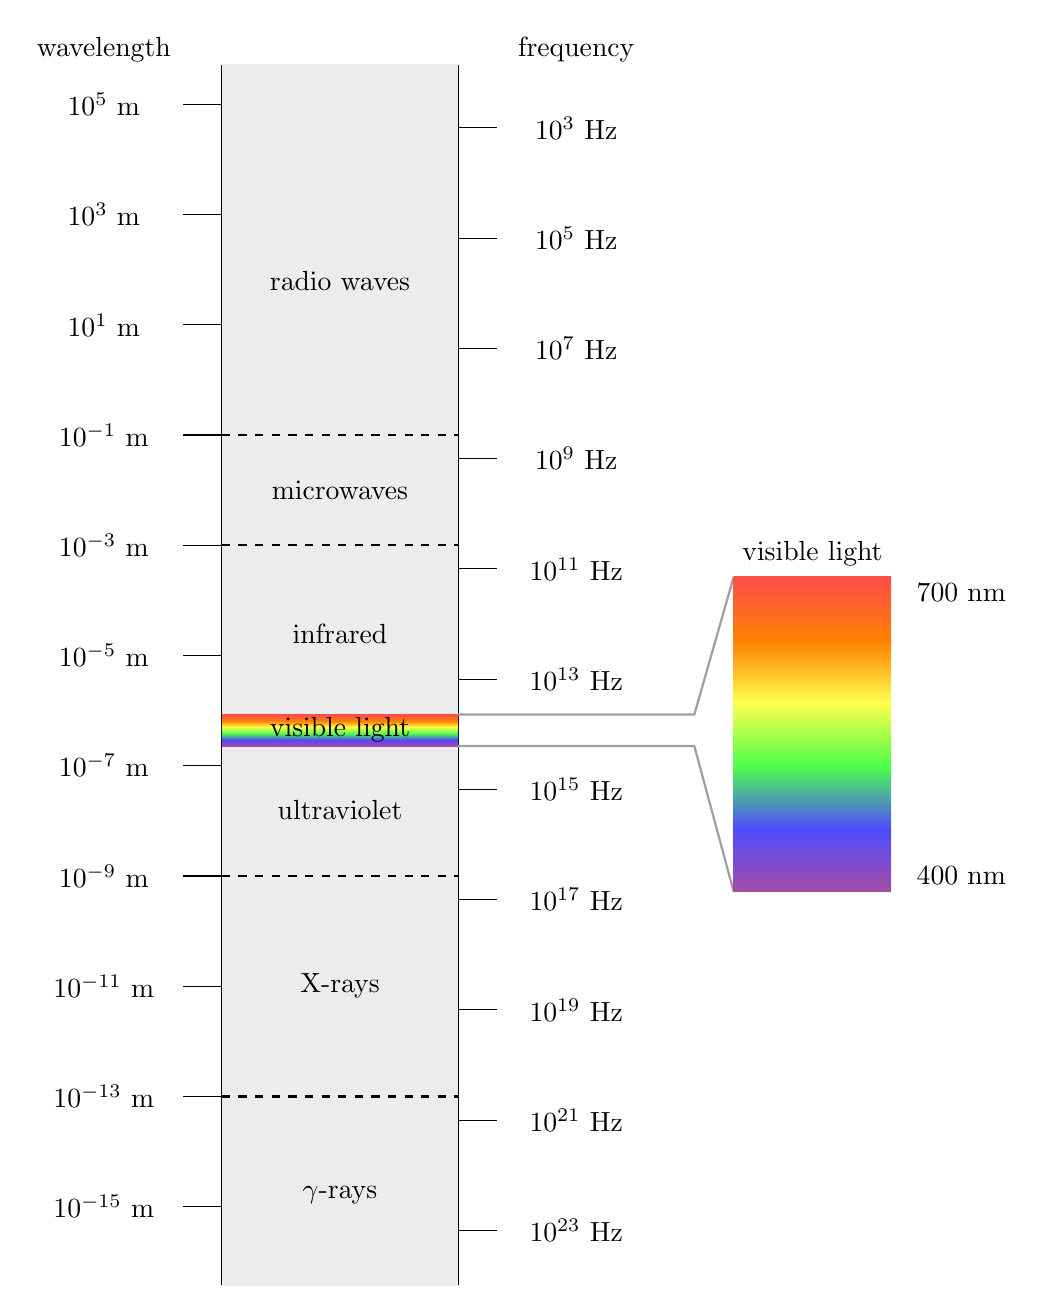
\begin{tikzpicture}
	% define visible spectrum shading
	\pgfdeclareverticalshading{visible}{100bp}
	{color(0bp)=(violet!70); color(25bp)=(violet!70); color(35bp)=(blue!70);
		color(45bp)=(green!70); color(55bp)=(yellow!70); color(65bp)=(orange);
		color(75bp)=(red!70); color(100bp)=(red!70)}
	% grayish background for spectrum labels
	\draw[gray!15,fill] (-1.5,-8) rectangle (1.5,7.5);
	% axes
	\draw (-1.5,-8) -- (-1.5,7.5) (1.5,-8) -- (1.5,7.5);
	\node at (-3,7.7) {wavelength};
	\node at (3,7.7) {frequency};
	% spectrum labels
	\shade[shading=visible] (-1.5,-1.15) rectangle (1.5,-0.75);
	\foreach \x/\xlabel in {1.8/{radio waves}, -2/{microwaves}, -4.6/{infrared}, -6.35/{visible light}, -7.8/{ultraviolet}, -11/{X-rays}, -14.8/{$\gamma$-rays} } \node at (0,{\x*0.7+3.5}) {\xlabel};
	% values of wavelengths
	\foreach \x in {5,3,1,...,-15} {
		\draw (-1.5,{\x*0.7+3.5}) --++ (-0.5,0);
		\node at (-3,{\x*0.7+3.5}) {$10^{\x}$ m};
	}
	% values of frequencies
	\foreach \x in {3,5,...,23} {
		\draw (1.5,{-\x*0.7+8.8}) --++ (0.5,0);
		\node at (3,{-\x*0.7+8.8}) {$10^{\x}$ Hz};
	}
	% dashed lines as separators
	\foreach \x in {-1,-3,-9,-13} \draw[dashed,thick] (-1.5,{\x*0.7+3.5}) --++ (3,0);
	% extension for visible spectrum
	\draw[thick, gray!75] (1.5,-1.15) --++ (3,0) -- (5,-3);
	\draw[thick, gray!75] (1.5,-0.75) --++ (3,0) -- (5,1);
	\shade[shading=visible] (5,-3) rectangle (7,1);
	\node at (6, 1.3) {visible light};
	\node[right] at (7.2, 0.8) {700 nm};
	\node[right] at (7.2, -2.8) {400 nm};
\end{tikzpicture}
\end{document}